% Modified 31 Oct 2005:  Conditioning fallacy alluded to.
% This chapter has been modified on 6-4-05.
% There are two \choice
\pagestyle{headings}
\setcounter{chapter}{0}
\chapter{Descriptive Statistics} \label{chp 1}
\setcounter{page}{1}

\section{Sampling}

\begin{definition}
Given a research question to be addressed by a study or experiment, the group that the question concerns is called a \newterm{population}\index{Population}. Our goal is to try to answer the question using data about some smaller subset of the population, known as a \newterm{sample}\index{Sample}.
\end{definition}

\begin{example}
We are interested in whether a new treatment for pollen allergies is more effective than an existing treatment. To try to answer this question, we can take a large group of people with pollen allergies, give half the new treatment, give the other half the existing treatment, and have them report their results so we can compare. 

We're interested in studying individuals with pollen allergies, in general, that's the population in this scenario. Only those who took one of the two treatments and reported their results back are members of the sample.
\end{example}

\begin{keypoint}
Someone who took one of the treatments, but did not report their results, is not in our sample. The sample is the group we have data about.
\end{keypoint}

Perhaps the simplest way to illustrate the distinction is to think of the population as the group we \emph{want to know about}, and the sample as the group we \emph{do know about}.

\begin{example}
A semiconductor fabrication plant wants to estimate the proportion of defective chips among their total production. To do this, they test every twentieth chip that leaves the production line.

Since they're interested in what proportion of all chips they produce are defective, the population here consists of all chips produced at their plant. The sample includes only those that are tested.
\end{example}

\subsection*{Statistics \& Parameters}

\begin{definition}
A numerical property of a population is called a \newterm{parameter}\index{Parameter}, while a numerical property of sample is called a \newterm{statistic}\index{Statistic}.
\end{definition}

\begin{example}
In a forest where $41.3\%$ of trees are cedar, a biologist (who is unaware of this fact) estimates the proportion of cedar trees by selecting twenty different trees in the forest at random. She notes that eleven of the twenty trees in her sample are cedar, so estimates that $\frac{11}{20} = 55\%$ of trees in the forest are cedar. In this context the value of $55\%$ she computes is a statistic, and the true value of $41.3\%$ is a parameter.
\end{example}

In some contexts, the distinction is more subtle. The point is to consider how a quantity relates to the question that it's being used to address. Does the value give a definitive answer based on complete information, with no uncertainty, or is it based on partial information or subject to some degree of uncertainty?

\begin{example}
LeBron James' free throw percentage in 2024 was $56.6\%$. If this figure is being used to answer the question `what was LeBron James' free throw percentage in 2024', then it's a parameter, but if it's being used to answer the question `how likely is LeBron James to make his next free throw' then it's a statistic.
\end{example}

\begin{remark}
Some quantities colloquially called statistics are not, in fact, statistics. If a college concludes that 23\% of its current students are enrolled in the science program by examining their complete records of student enrollment, they haven't computed a statistic, they've computed a parameter.
\end{remark}

The discipline of statistics is about making decisions using sample data. There are so many contexts where sample data is the only kind of information or the highest quality kind of information we have access to, which is why the applications of statistics are so varied.

Given a research question, and relevant sample data, the first question to ask is: how was the sample obtained? Our ability to do statistics well depends on one factor more than any other: do we have an accurate model of the sampling process? In other words, do we understand the process that generated the data we're working with?

\subsection*{Three Kinds of Samples}

\begin{definition}
If we take as our sample those members of the population that are easiest to access, we obtain a \newterm{convenience sample}\index{Convenience Sample}. \\ If we order our population in some way and periodically select members at regular intervals, we obtain a \newterm{systematic sample}\index{Systematic Sample}. \\ If we select members of the population at random, with all members having an equal chance of appearing on every selection, we obtain a \newterm{simple random sample}\index{Simple Random Sample}.
\end{definition}

\begin{remark}
Sampling can be done \newterm{with replacement}\index{Sampling!with replacement}, which means the same individual may appear many times in the sample, or \newterm{without replacement}\index{Sampling!without replacement}, which means that each individual can appear at most once in the sample.

Think about this process for generating a simple random sample: we put the names of every individual in our population (supposing these are unique) into a hat and draw names. When sampling with replacement, after drawing a name we write it down, put it back in the hat, and shake the hat. When sampling without replacement, the names that are drawn are not put back into the hat.
\end{remark}

In the rest of the course, whenever we refer to a random sample, this will be shorthand for a simple random sample taken with replacement. This means the sampling process is equivalent to repeatedly rolling a die labelled with the names of the members of our population, with the outcome of any one roll having no effect on the outcome of any other. This will allow us, later on in the course, to provide precise justifications and error bounds for our estimates and predictions by applying the theory of probability.

\begin{warning}
In colloquial language, the term random sample could be interpreted as a sample derived from an unknown or not well-understood process. In statistics, a random sample (a simple random sample taken with replacement) results from a completely specified process, namely, drawing names from a hat in manner where each name is equally likely to appear on each selection, regardless of which names are drawn before or after, or repeatedly rolling a die where each side corresponds to a different individual in the population.
\end{warning}

\begin{example}
A semiconductor fabrication plant wants to estimate the proportion of defective chips among their total production. To do this, they test every twentieth chip that leaves the production line.

In this context, the sample obtained will be a systematic sample, not a random sample. If they select a random number between zero and twenty and start testing every twentieth chips after that many chips have been produced, they will still not obtain a random sample, since a sample which contains two consecutively produced chips cannot occur.
\end{example}

\begin{example}
In her statistics class, Anne is doing a project where she wants to estimate how many hours per week students in her age group spend commuting to and from school. She gathers data by asking ten of her friends about their commuting routine. 

In this case, Anne will obtain a convenience sample. Conclusions she draws about students in her age group are dubious, since she's only sampling students she happens to be close with.
\end{example}

Notice that in practice, it's often very difficult to obtain a random sample. It requires a complete list of all members of the population under study, and if these members are people, a way to guarantee they will volunteer the information the experimenters are interested in knowing. If you read any corporate software license agreement, you will almost certainly see a section which affirms all your user data is accessible for studies carried out by the company that developed the software. This ensures the company can obtain high quality samples from the population of its users.

An interesting sampling case study is the COVID-19 outbreak on the MV Diamond Princess, which was quarantined in February 2020. Under normal circumstances, there's no way to obtain a sample of people who are known to have been exposed to a disease (and may or may not have any symptoms), as we cannot forcibly expose people for ethical reasons, and subjects cannot self-select because those who are asymptomatic are often unaware they've been exposed at all. Because no one was allowed to leave the ship, researchers were able to derive accurate estimates of parameters like the proportion of COVID-19 cases which present as asymptomatic.

\section{Variables \& Levels of Measurement}

\begin{definition} 
The members of the population are referred to as \newterm{individuals}\index{Individuals}. Any property of these individuals which can take different values for different individuals is called a \newterm{variable}\index{Variable}.
\end{definition}

\begin{center}
\begin{tabular}{c|c|c|c|c}
Model & Year & Colour & Mileage & Condition \\ \hline
Toyota Yaris & 2015 & Blue & 85\,000 & B \\
Honda CRV & 2018 & Black & 140\,000 & C \\
Ford F-150 & 2022 & Red & 46\,000 & A \\
Subaru Outback & 2019 & Blue & 77\,000 & B \\
\end{tabular}
\end{center}

Typically, if we represent our data in a table, as above, each individual corresponds to a row of the table (in this case the individuals are used cars in some car seller's inventory), and each variable corresponds to a column. Variables can describe any aspect of the individuals in the data set. It's often useful to categorize them based on which operations we can meaningfully apply.

\begin{remark}
In statistics, the letter $n$ is reserved for the sample size, that is, the number of individuals in the dataset, and will appear frequently in formulas and explanations. In the dataset above, $n=4$.
\end{remark}

\begin{definition}
As we answer the three questions below, each affirmative answer moves the variable one level up in the hierarchy of \newterm{levels of measurement}\index{Levels of Measurement}.
$$\textbf{Categorical} \ \to \ \textbf{Ordinal} \ \to \ \textbf{Interval} \ \to \ \textbf{Ratio}$$
\begin{itemize}
\item Can we naturally order the values? (The $<$ and $>$ operations are meaningful)
\item Can we subtract and average the values? (The $+$ and $-$ operations are meaningful)
\item Can we multiply and divide the values? (The $\cdot$ and $\div$ operations are meaningful)
\end{itemize}
\end{definition}

\noindent\textbf{\emph{Ratio}}: Variables like height, distance, or anything else you can measure with a ruler, are at the ratio level. They are naturally ordered and we can perform arithmetic with them. In particular, ratios are meaningful. One distance can be twice as far as another, or two-thirds as far.

\noindent\textbf{\emph{Interval}}: Variables like shoe size or temperature (in\,$\,^{\circ} C$) are at the interval level. Ratios of values are not meaningful. The shoe size 8 is not twice as large as 4, and 10$\,^{\circ} C$ is not twice as hot as 5$\,^{\circ} C$. Values can be put a scale with equal increments, so we can form differences, say a difference of 5$\,^{\circ} C$ between two temperatures, and also compute averages.

\noindent\textbf{\emph{Ordinal}}: Variables like letter grade or level of satisfaction (very unsatisfied, unsatisfied, neutral, satisfied, or very satisfied) are at the ordinal level. None of the four basic arithmetic operations ($+$, $-$, $\cdot$, $\div$) are meaningful, but there's a clear natural ordering.

\noindent\textbf{\emph{Categorical}}: Variables like name, location, or colour are at the categorical level. The values of the variable have no natural ordering, they are simply labels that can be used to group individuals into categories.

In the case of our used car data in the table above, Model and Colour are at the categorical level, Condition is at the ordinal level, Year is at the interval level, and Mileage is at the ratio level.

\begin{note}
This system of classification of variables into four groups is widespread, but not universal. There are alternative systems, but the one described above is widely known and over time has become part of standard statistical vocabulary.
\end{note}

%Examples

\section{Histograms}

Any variable, regardless of its level of measurement, has some collection of values it may take, and each of these values occurs some number of times in the data. This information, taken all together, constitutes the \newterm{distribution} of the variable. The most intuitive way to understand the distribution of a variable is often through a \newterm{histogram}\index{Histogram}.

\begin{center}
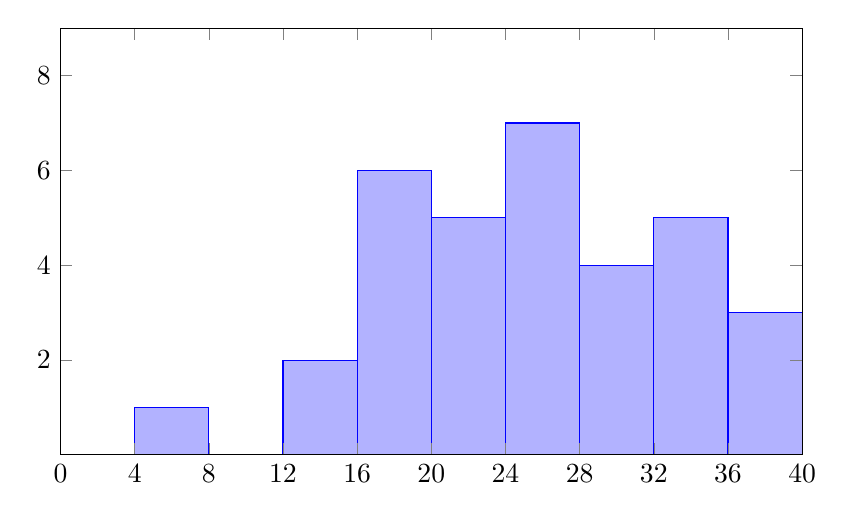
\begin{tikzpicture}
    \begin{axis}[
        width=11cm,
        height=7cm,
        xmin=0, xmax=40,
        ymin=0, ymax=9,
        xtick distance=4,
        ytick = {2,4,6,8},
        area style,
    ]
    \addplot+[ybar interval] plot coordinates { (0,0) (4,1) (8,0) (12,2) (16,6) (20,5) (24,7) (28,4) (32,5) (36,3) (40,1)};
\end{axis}
\end{tikzpicture}
\end{center}

The horizontal axis, which represents the variable's value, is divided into segments of equal width, known as \newterm{bins} or \newterm{classes}, and the height of each bar is the number of individuals whose values fall into that particular bin. Each bin has a \newterm{lower limit} and an \newterm{upper limit}. The distance between consecutive lower limits is called the \newterm{bin width} or \newterm{class width}.

The above discussion only applies to variables at the interval or ratio levels of measurement. When we don't have a scale which can be divided into segments of equal width, we can instead create one bin for each possible value of the variable, and the result is usually called a \newterm{bar graph}.

\begin{example}\label{FirstHistogram}
Create a histogram with five bins, to visualize the distribution of ages in a room of kids whose ages are given, in order, below.
$$2\ \ 3\ \ 3\ \ 4\ \ 5\ \ 5\ \ 6\ \ 7\ \ 7\ \ 7\ \ 7\ \ 7\ \ 7\ \ 8\ \ 8\ \ 9\ \ 9\ \ 10\ \  11\ \ 11\ \ 11\ \ 12 \ \ 14$$
We need to partition these 23 values into five bins of equal width. One way to do this is to compute the \newterm{range} of the data (the difference between the smallest and largest value), then add one and divide that by the number of bins, in this case, five.

This calculation yields $\frac{14-2+1}{5} = 2.6$, which we'll round up to 3, and take as the bin width. Adding one to the range and always rounding up will ensure the largest value doesn't exceed the upper limit of the last bin. Taking the smallest data value as the lower limit of the first bin, and repeatedly adding the bin width to obtain the lower limits of the other bins gives the table and histogram below. 

\begin{center}
\begin{tabular}{|c|c|c|c|c|c|}
\hline
Bins & \,$2 - 4$\, & \,$5 - 7$\, & \,$8 - 10$ & $11 - 13$ & $14 - 16$ \\
\hline
Counts & $4$ & $9$ & $5$ & $4$ & $1$ \\
\hline
\end{tabular}
\end{center}

\begin{center}
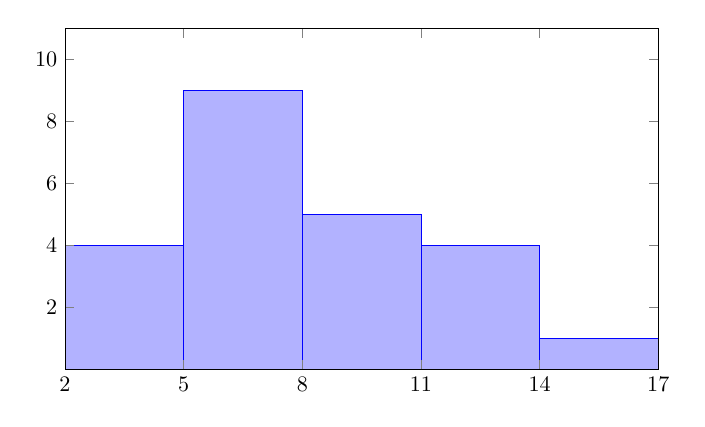
\begin{tikzpicture}[scale=0.8]
    \begin{axis}[
        width=11cm,
        height=7cm,
        xmin=2, xmax=17,
        ymin=0, ymax=11,
        xtick = {2,5,8,11,14,17},
        ytick = {2,4,6,8,10},
        area style,
    ]
    \addplot+[ybar interval] plot coordinates { (2,4) (5,9) (8,5) (11,4) (14,1) (17,0) };
\end{axis}
\end{tikzpicture}
\end{center}
\end{example}

The precise details of the process that creates the bins is not important, as long as the horizontal axis is divided into consecutive segments of equal width in a way that gives a useful visualization of the distribution of the variable.

\begin{example}
Consider the first eleven positive integers. The histogram below on the left was created from these values by using 2.2 for the bin width, and 0.2 for the lower limit of the first bin. The histogram below on the right was created from the same values by using 1.9 for the bin width, and 1 for the lower limit of the first bin.
\begin{center}
\begin{minipage}{0.47\textwidth}
\centering
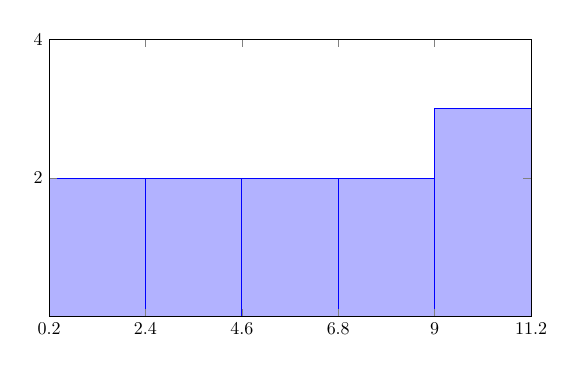
\begin{tikzpicture}[scale=0.65]
    \begin{axis}[
        width=11cm,
        height=7cm,
        xmin=0.2, xmax=11.2,
        ymin=0, ymax=4,
        xtick = {0.2,2.4,4.6,6.8,9,11.2},
        ytick = {2,4,6,8,10},
        area style,
    ]
    \addplot+[ybar interval] plot coordinates { (0.2,2) (2.4,2) (4.6,2) (6.8,2) (9,3) (11.2,0)};
\end{axis}
\end{tikzpicture}
\end{minipage}
\begin{minipage}{0.47\textwidth}
\centering
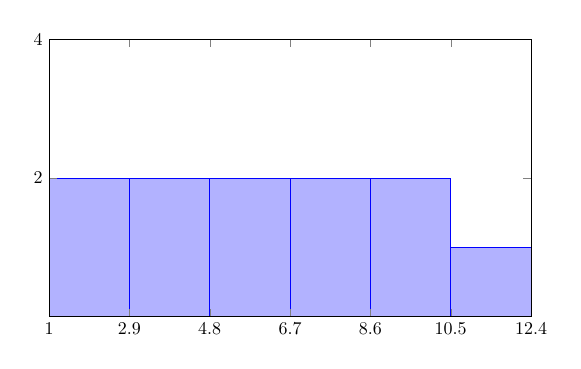
\begin{tikzpicture}[scale=0.65]
    \begin{axis}[
        width=11cm,
        height=7cm,
        xmin=1, xmax=12.4,
        ymin=0, ymax=4,
        xtick = {1,2.9,4.8,6.7,8.6,10.5,12.4},
        ytick = {2,4,6,8,10},
        area style,
    ]
    \addplot+[ybar interval] plot coordinates { (1,2) (2.9,2) (4.8,2) (6.7,2) (8.6,2) (10.5,1) (12.4,0) };
\end{axis}
\end{tikzpicture}
\end{minipage}
\end{center}

There is nothing incorrect about either of the two histograms, it's simply a quirk of the way the axis was divided into bins that results in the difference in appearance. This illustrates how it's sometimes possible to build intentional bias into a histogram.
\end{example}

As mentioned above, we won't dwell on the details of the process of creating bins, but suffice to say it is good practice to have some consistent, explicit process (usually the one built-in to whatever software package is being used to generate the histogram) and not tweak the details until the result is deemed satisfactory, which one might call `bin hacking'.

%\begin{note}
%If a data value lies exactly on the boundary of two bins, it has be put into one or the other. This decision should always be made the same way (either all values on the boundary are put in the smaller bin, or all values on the boundary are put in the larger bin) when creating a histogram.
%\end{note}

%Idea of a distribution

%Examples of Histograms

%Example where choosing different boundaries on categories gives a different impression

\section{Measures of Center}\label{MeasuresOfCenterSec}

It's often useful to give a description of where the middle of a distribution lies by producing a single `typical' or `central' value. The mean, median, and mode are the most common methods of producing such a value.

\begin{definition}
Let $x_1, x_2,\,\dots\,, x_n$ be values of a statistical variable that occur across the $n$ individuals in a dataset.
\begin{itemize}
\item The \newterm{mean}\index{Mean} value of the variable is given by $\frac{1}{n}\sum_{i} x_i = \frac{1}{n}(x_1 + x_2 + \dots + x_n)$.
\item The \newterm{median}\index{Median} value of the variable is obtained by ordering $x_1, x_2, \dots\,, x_n$ smallest to largest, then taking the value in the middle of the resulting list if $n$ is odd, and the mean of the two values nearest the middle if $n$ is even.
\item The \newterm{mode}\index{Mode} is the value of the variable which occurs most frequently in the data. If no value occurs more than once, we say the variable has no mode. Note that there may be more than one mode.
\end{itemize}
\end{definition}

\begin{example}
Consider the set of values $1,1,2,3,5$. We can compute the mean $\frac{1}{5}(1+1+2+3+5) = 2.4$, and since the values are already given in sorted order, we can see the median is $2$ and the mode is $1$.
\end{example}

Note that these three measures of centre correspond to three levels or measurement. The mean is defined at the interval level and above, the median is defined at the the ordinal level and above, and the mode is defined even at the categorical level.

\begin{warning}
In colloquial language, the average almost always refers to the mean, but there are many situations where it doesn't. The average letter grade cannot refer to the mean, since letter grades are ordinal data, and income and wealth averages quoted in the media are often medians, not means.
\end{warning}

Here's a scenario that illustrates the relevance of each measure: In a guessing game, five numbered balls are put into an urn. The distribution of numbers matches our data in the last example (two balls labelled with 1, one with 2, one with 3, and one with 5). A ball is drawn at random from the urn, and the player's task is to guess the number the ball will be labelled with.

If there is a \$10 reward for guessing correctly, and no payout for guessing incorrectly, clearly the best strategy is to guess the mode, $1$. What's not so immediate is that if instead the player is rewarded \$10 minus the error in their guess (so guessing 3 then drawing a 5 will yield a reward of $10 - 2 = 8$ dollars), the best strategy is to guess the median, 2, and if the player is rewarded \$10 minus the squared error in their guess (so guessing 3 then drawing a 5 will yield a reward of $10 - 2^2 = 6$ dollars), then the best strategy is to guess the mean, 2.4. 

This is not a quirk that happens because of the particular choice of labels on the balls. In general, regardless of the distribution of values, \emph{the median minimizes the average absolute error} and \emph{the mean minimizes the average squared error}. These results can be stated formally and proven in the language of random variables (which we'll get to in Chapter 4) with techniques from differential calculus.

\begin{example}
In the preceding section, we constructed the histogram shown below to summarize the distribution of the variable whose values were as follows.
$$2\ \ 3\ \ 3\ \ 4\ \ 5\ \ 5\ \ 6\ \ 7\ \ 7\ \ 7\ \ 7\ \ 7\ \ 7\ \ 8\ \ 8\ \ 9\ \ 9\ \ 10\ \  11\ \ 11\ \ 11\ \ 12 \ \ 14$$
\begin{center}
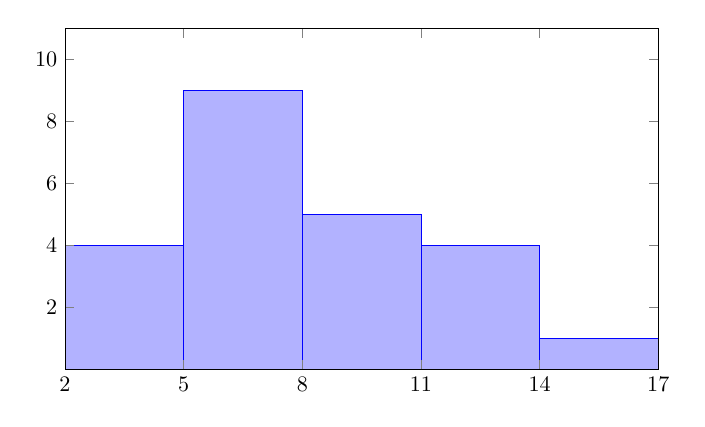
\begin{tikzpicture}[scale=0.8]
    \begin{axis}[
        width=11cm,
        height=7cm,
        xmin=2, xmax=17,
        ymin=0, ymax=11,
        xtick = {2,5,8,11,14,17},
        ytick = {2,4,6,8,10},
        area style,
    ]
    \addplot+[ybar interval] plot coordinates { (2,4) (5,9) (8,5) (11,4) (14,1) (17,0) };
\end{axis}
\end{tikzpicture}
\end{center}
There are $23$ values in the ordered list, so the median is the $12^{th}$ value, which is a 7, while the mean is $\frac{1}{23}(2 + 3 + 3 + \dots + 14) = 7.57$. Notice that the mean is a little bit larger than the median. When the distribution of a variable has a longer tail on one side, the mean is pulled towards the tail more than the median.
\end{example}

The most extreme form of this effect occurs when a data value which is much larger than or much smaller than all the other values is present. Such values could occur by mistake, as typos, or could occur because of the nature of the population that the data was sampled from.

\begin{keypoint}
Adding an extra value (or two, or three) to a dataset which is very different from the rest, that is, adding an \newterm{outlier}\index{Outlier}, will affect the mean more than the median. It's common to summarize this by saying the median is more \emph{stable} than the mean.
\end{keypoint}

For this reason, I encourage students to pay more attention to the median grades in their classes than the mean grades. If a few students miss a test and receive a zero, this can have a noticeable effect on the mean, and give students a false impression of where they stand relative to their classmates. Students are also often concerned about whether their grade ranks them among the top half of the class, which is a question the median answers, not the mean.

In general, if the data being studied contains outliers, the median is often preferred over the mean. This is why it's more common to measure median income than mean income. The distribution of income has such a long tail that citing the mean income can be deceptive when studying populations with high income inequality.

\begin{example}
Mr.\,Brown's grade three class has fifteen students, and the mean height in his class is 117\,cm. Mrs.\,Green's grade three class has twelve students, and the mean height in her class is 122\,cm. What is the mean height in the combined group of twenty-seven students?

We know that $\frac{S_B}{15} = 117$ and $\frac{S_G}{12} = 122$, where $S_B$ and $S_G$ are the sums of the heights of all students in Mr.\,Brown's and Mrs.\,Green's classes, respectively. Therefore, $S_B = 15 \cdot 117$ and $S_G = 12\cdot 122$. We can then calculate the mean of the entire group as
$$\frac{S_B + S_G}{27} = \frac{15\cdot 117 + 12 \cdot 122}{27} = 119.22.$$
\end{example}

The example above, and the one below, are typical of more involved problems about means, which often require you to pass from a mean to the corresponding sum. You should get used to doing this, as the same idea will reappear later in the course when we study the central limit theorem.

\begin{example}
Mr.\,Brown's grade three class has fifteen students, and the mean height in his class is 117\,cm. If a new student who is 114\,cm tall joins the class, how will the mean change?

As above, we know that $\frac{S_B}{15} = 117$, so $S_B = 15 \cdot 117$. We can then calculate the mean of the new group of sixteen students as below, and conclude the mean height will drop by 0.19\,cm.
$$\frac{S_B + 114}{16} = 116.81$$
\end{example}

\begin{remark}
It will be extremely important to distinguish the mean of a population from the mean of a random sample taken from a population. For this reason, the greek letter $\mu$ is used for the mean of a population (a parameter), while $\littlexbar$ is used for the mean of a sample (a statistic). It is standard practice to reserve greek letters for parameters to keep the parameter / statistic distinction clear.
\end{remark}

\begin{example}
A random number generator produces the values $1$, $2$, $3$, $4$, $5$, and $6$ with equal probability. Three random numbers are produced, and the results are $2$, $2$, and $5$.

The mean value generated by the random number generator is $\mu = \frac{1}{6}(1+2+3+4+5+6) = 3.5$, while the mean in the sample of three values is $\littlexbar = \frac{1}{3}(2+2+5) = 3$.
\end{example}
%Examples

%Exercise for the reader: show these minimize different expectations <- Later!

\section{Measures of Dispersion}\label{MeasuresOfDispersionSec}

\begin{center}
\begin{minipage}{0.47\textwidth}
\centering
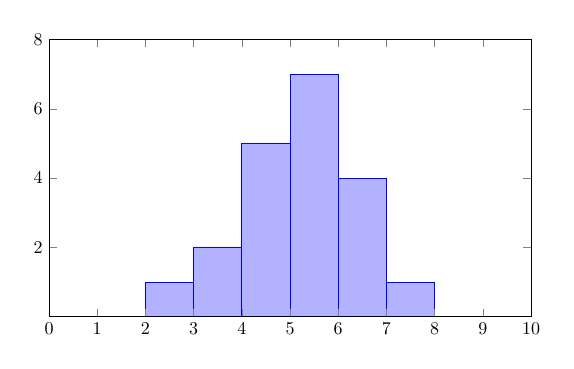
\begin{tikzpicture}[scale=0.65]
    \begin{axis}[
        width=11cm,
        height=7cm,
        xmin=0, xmax=10,
        ymin=0, ymax=8,
        xtick = {0,1,2,3,4,5,6,7,8,9,10},
        ytick = {2,4,6,8,10},
        area style,
    ]
    \addplot+[ybar interval] plot coordinates { (0,0) (1,0) (2,1) (3,2) (4,5) (5,7) (6,4) (7,1) (8,0) (9,0) (10,0)};
\end{axis}
\end{tikzpicture}
\end{minipage}
\begin{minipage}{0.47\textwidth}
\centering
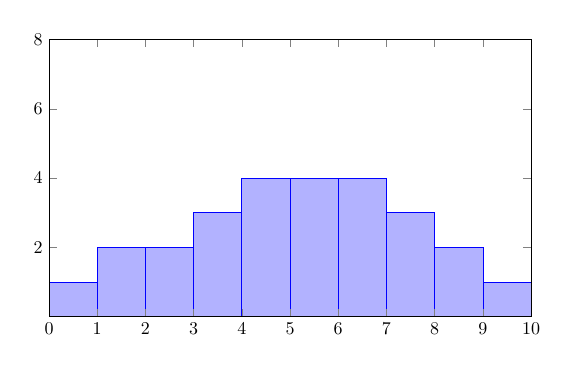
\begin{tikzpicture}[scale=0.65]
    \begin{axis}[
        width=11cm,
        height=7cm,
        xmin=0, xmax=10,
        ymin=0, ymax=8,
        xtick = {0,1,2,3,4,5,6,7,8,9,10},
        ytick = {2,4,6,8,10},
        area style,
    ]
    \addplot+[ybar interval] plot coordinates { (0,1) (1,2) (2,2) (3,3) (4,4) (5,4) (6,4) (7,3) (8,2) (9,1) (10,0)};
\end{axis}
\end{tikzpicture}
\end{minipage}
\end{center}

The two distributions pictured in the histograms above have a similar mean, somewhere between 5 and 6 in both cases, but differ noticeably in how the data is distributed around the mean. The variable whose distribution is pictured on the right is more likely to take values farther from it's mean. We say it has higher \newterm{dispersion} than the variable on the left. In this section we'll introduce a few ways to quantify this notion.

We could measure dispersion by simply taking the difference between the smallest and largest data values. This is known as the \newterm{range}\index{Range} of the variable. However, the range is extremely sensitive to outliers, and ignores almost all of the data (all but the largest and smallest values). We can do better.

\begin{definition}
Let $Q_1$ denote the median of all values smaller than the median, and let $Q_3$ denote the median of all values larger than the median. These are known, respectively, as the first and third quartile\index{Quartiles}. The \newterm{interquartile range}\index{Interquartile Range} is given by $IQR = Q_3 - Q_1$.
\end{definition}

The idea here is to divide the sorted data into blocks: the smallest $25\%$, the middle $50\%$, and the largest $25\%$. The interquartile range is the width of the middle block. This is a quick way to quantify dispersion, which as with median, is not strongly influenced by the presence of outliers.

\begin{example}
Calculate median and IQR of the variable that takes the values below. 
$$1\ \ 1\ \ 2\ \ 4\ \ 7$$
The values are already in sorted order, so we can see the median is $2$, and the first and third quartiles are $Q_1 = \frac{1+1}{2} = 1$, and $Q_3 = \frac{4+7}{2} = 5.5$. Then $IQR = 5.5 - 1 = 4.5$.
\end{example}

Although the interquartile range is useful for summarizing data, by far the most important measure of dispersion in statistical theory and practice is the variance, together with its square root, the standard deviation.

\begin{definition}\label{VarianceDef}
The average squared distance from the mean is called the \newterm{variance}\index{Variance! of a Population}, and denoted $\sigma^2$. If $x_1, x_2,\,\dots\,, x_n$ are the values of a statistical variable that occur across the $n$ individuals in the dataset, and $\mu$ is the mean of these values, then the variance is given by $\sigma^2 = \textstyle\frac{1}{n}\sum_{i=1}^{n}(x_i - \mu)^2$. The square root of the variance, $\sigma$, is known as the \newterm{standard deviation}.\index{Standard Deviation! of a Population}
\end{definition}

\begin{example}
Find the variance and standard deviation of the variable that takes the values below. 
$$1\ \ 1\ \ 2\ \ 4\ \ 7$$
First we compute $\mu = \frac{1}{5}(1+1+2+4+7) = 3$. Then we can calculate the variance as
$$\sigma^2 = \textstyle\frac{1}{5}[(1-3)^2+(1-3)^2+(2-3)^2+(4-3)^2+(7-3)^2] = \frac{1}{5}[4+4+1+1+16] = \frac{26}{5},$$
and the standard deviation is $\sigma = \sqrt{\frac{26}{5}}=2.28$.
\end{example}

\begin{warning}
The standard deviation is not the average distance from the mean. We know that $\sqrt{a^2 + b^2} \neq a + b$, and similarly, the average of a sequence of terms is not generally the same as the square root of the average of their squares.

The actual average distance from the mean is known as the mean absolute deviation\index{Mean Absolute Deviation}, which we will not study in this course. It's a fine measure of dispersion, but does not play as central a role in statistics as the variance and standard deviation do.
\end{warning}

%Note: Percentiles in R.V. section along with CDFs

%Examples

%Def: Variance, Sample Variance, 

\subsection*{Bessel's Correction}

%Typically, when we measure some property of a sample, the point is to use that information as an estimate of the corresponding property of the population. To get an idea of what the mean age is in a certain geographic area, we can take a random sample, calculate the mean age in the sample, and use that statistic as an estimate.

%This process seems completely natural, however, there's a lot of subtlety hiding here. If we take the variance in a random sample as an estimate of the variance in the population the sample was drawn from, it turns out that, on average, we will be underestimating.

Suppose we want to determine the age of the oldest person in a population, and we do so by taking a random sample, and using the age of the oldest person in the sample as our estimate. It should be clear that, typically, the result will be an underestimate. Why? This process will certainly never produce an overestimate, and unless the random sample happens to contain the oldest person in the population, or someone else of the same age, the estimate will be too low. Thus, if we average over all possible samples, the value of our estimate will be lower than the actual age of the oldest person in the population.

This problem doesn't occur when using the sample mean to estimate the population mean. It turns out that the average value of the sample mean, across all possible samples, is always precisely equal to the population mean (we say the sample mean is an \newterm{unbiased estimator}\index{Unbiased Estimator} of the population mean, while the sample maximum is a \newterm{biased estimator}\index{Biased Estimator} of the population maximum). These notions are developed rigorously in the Probability \& Random Variables option course, 201-PRV.

Unfortunately, if we calculate the variance in our sample using the formula introduced earlier, this results in a biased estimator of the population variance, which undershoots on average. The good news is that we can fix the problem easily, and obtain an unbiased estimator for the population variance, by making a small change in the way we calculate the variance of a sample, called Bessel's correction, after German astronomer and mathematician Friedrich Bessel.

\begin{definition}\index{Sample Standard Deviation}\index{Standard Deviation! of a Sample}\index{Variance! of a Sample}\index{Bessel's Correction}\label{SampleStdDev}The (Bessel corrected) \newterm{sample variance} is $s^2 = \frac{1}{n-1}\sum_{i} (x_i - \overline{x})^2$ and the (Bessel corrected) \newterm{sample standard deviation}, $s$, is its square root.
\end{definition}

There are two important changes to note. First, the mean is denoted $\littlexbar$, since we're working with sample data, and second, instead of averaging as usual, by dividing by the number of terms in the sum, we decrease the divisor by one. This is Bessel's correction.

\begin{example} 
Find the mean and sample variance of the sample of five values $2$, $0$, $7$, $3$, $3$.
$$\littlexbar = \textstyle\frac{1}{n}\sum_{i} x_i = \frac{1}{5}(2+0+7+3+3) = 3$$
$$s^2 = \textstyle\frac{1}{n-1}\sum_{i} (x_i - \overline{x})^2 = \frac{1}{4}[(-1)^2+(-3)^2+(4)^2+(0)^2+(0)^2] = \frac{13}{2}$$
\end{example}

In practice, the Bessel corrected variance and standard deviation are used almost universally. Try calculating the standard deviation of a small list of values using spreadsheet software on a computer. You'll find two commands to calculate the standard deviation, one where Bessel's correction is applied (STDEV.S in Excel or Google Sheets) and one where it isn't (STDEV.P in Excel or Google Sheets). 

\begin{remark}
Sample variance and sample standard deviation always refer to the Bessel corrected values. When referring to the formula in Definition \ref{VarianceDef}, we'll omit the prefix sample, or sometimes explicitly use the terms population variance or population standard deviation to be as clear as possible.
\end{remark}

\begin{example}
Consider a standard fair six-sided die. Find the mean and variance for the outcome of a single die roll. Find the mean and variance for a sample of four rolls whose results are $2$, $3$, $6$, $1$.

Treating the list of values $1$, $2$, $3$, $4$, $5$, $6$ as a complete population, we have
$$\mu = \textstyle\frac{1}{6}(1+2+3+4+5+6) = 3.5$$
$$\sigma^2 = \textstyle\frac{1}{6}[(-2.5)^2+(-1.5)^2+(-0.5)^2+(0.5)^2+(1.5)^2+(2.5)^2] = \frac{35}{12}.$$

From the sample of values $2$, $3$, $6$, $1$, we have
$$\littlexbar = \textstyle\frac{1}{4}(2+3+6+1) = 3$$
$$s^2 = \textstyle\frac{1}{3}[(-1)^2+(0)^2+(3)^2+(2)^2] = \frac{14}{3}.$$
\end{example}




